\documentclass[titlepage, 13px, a4paper]{report}

\usepackage[utf8]{inputenc}

\usepackage[T1]{fontenc}
\usepackage{fontawesome}
\usepackage{eurosym}

\usepackage[french]{babel}

\usepackage{fancyhdr}
\usepackage{graphicx}
\usepackage[left=4cm,right=4cm,top=4cm,bottom=5cm,textheight=25cm]{geometry}
\usepackage{wrapfig}

\usepackage{eso-pic}
\usepackage{transparent}

\usepackage{hyperref}
\usepackage{setspace}

\usepackage{titletoc}

%\usepackage{titlesec}
%\titleformat{\part}[display]
  %{\normalfont\bfseries}{}{0pt}{\Large\bfseries}

\newcommand\BackgroundPic{%
	\put(0,-50){%
		\parbox[b][\paperheight]{\paperwidth}{%
			%\vfill
			\centering
			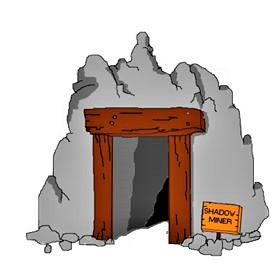
\includegraphics[%
			keepaspectratio]{../../images/icone.jpg}%
			\vfill
		}
	}
}

  
\renewcommand{\baselinestretch}{1.15}
\renewcommand{\partname}{}

\title{\textbf{{\Huge Rapport de soutenance \no 2}}}
\author{
	\\
	\bsc{{\LARGE ACCEr}} \\ \\
	\bsc{{\LARGE ShadowMiner}} \\ \\ \\
	\bsc{CLAUDEL Antoine} \\
	\bsc{FARINAZZO Cédric} \\
	\bsc{LANGUERRE Clément} \\
	\bsc{GRIZZI Edgar} \\ \\ \\
}
\date{{\LARGE \today}}

\pagestyle{fancy}
\fancyfoot[L]{
\includegraphics{../../images/ShadowMiners_logo_mini.png}} %50x33
\fancyhead[R]{ACCEr}
\fancyhead[L]{Rapport de soutenance \no 2}

\begin{document}
\AddToShipoutPicture*{\BackgroundPic}

\maketitle
\tableofcontents




\newpage 
\section{Introduction} 
\paragraph{} \hspace{0pt} 
Le projet « ShadowMiner » est un jeu vidéo d'épouvante conçu par le
groupe ACCEr. Le groupe est composé d'Antoine CLAUDEL, Cédric FARINAZZO, Clément LANGUERRE
et Edgar GRIZZI, quatre étudiants en cycle préparatoire InfoSup à EPITA. \\ \\
Le projet a débuté le 1er janvier 2018 et sera terminé en juin 2018. \\ \\
Le jeu vidéo a été conçu à l'aide du framework Unity (site web : \url{https://unity3d.com/fr]} ). 
Ce rapport décrit l'avancement dans la création du jeu de la première soutenance du 16
mars à la seconde soutenance du 04 mai. \\ \\
En premier lieu nous aborderons l'avancement général en rappelant les anciens objectifs fixés lors de la
première soutenance, en indiquant la réussite partielle ou totale de ces
objectifs et en donnant les nouveaux objectifs pour la dernière soutenance. \\
En second lieu nous mentionnerons les problèmes rencontrés, les apports
collectifs et individuels du groupe et les points de vue de chacun. \\
Enfin nous conclurons ce rapport avec des images provenant du jeu et les sources des
outils ou médias utilisés dans le cadre du projet.




\newpage




\fancypagestyle{plain}{}
\part{Avancement général}  
\section{Les objectifs remplis} 
\paragraph{} \hspace{0pt} 
Entre cette soutenance et la précèdente, nous avons eu plus de temps. Nous avons pu bien avancer notre jeu. \\
Il a bien évolué depuis la première soutenance où nous avions juste 2 niveaux et un début de multijoueurs.
Désormais, nous avons un beau menu, avec des niveaux solos, des paramètres fonctionnels et un mode multijoueur amélioré.

{\begin{enumerate}
	\item Nous avons créé quelques préfabs tels que des clés ou des pépites d'or afin d’améliorer nos niveaux 
			et plonger dans un univers ressemblant le plus possible à une mine.	\\
	\item Nous avons amélioré notre site internet afin de pouvoir créer un pseudo pour chaque utilisateur qui est Bob par défaut.	\\
	\item Ainsi nous avons créé un serveur en C\# connecté à la base de données (MySql) du site web \url{https://accer.ddns.net/}
			et un client en C\# intégré au jeu. 
			Ce serveur et ce client communiquent entre eux sur le port 4247 avec le protocole TCP et permettent à l’utilisateur de créer, se connecter ou
			manager son compte directement depuis le jeu. \\
			Ainsi les comptes créés depuis le jeu sont aussi accessibles sur le site avec les mêmes identifiants. \\
	\item Nous avons revu notre menu. Il comporte 6 boutons :
		{\begin{itemize}
			\item	Un bouton pour jouer au mode solo
			\item	Un bouton pour jouer au mode multijoueurs
			\item	Un bouton pour ouvrir le site web dans un navigateur web
			\item	Un bouton pour accéder au menu des comptes
			\item	Un bouton pour quitter le jeu. \\
		\end{itemize}} 
	\item Un menu des paramètres a été ajouté afin de modifier la qualité des graphismes, la résolution de la fenêtre, 
		l’activation ou la désactivation du mode plein écran, de changer la fréquence d’affichage, de régler la sensibilité de la souris, 
		de changer les touches, de changer le volume sonore de la musique et des effets sonores. \\
	\item Une série de scènes permettant de créer son compte ,de s'y connecter ou de le gérer, a été créée en lien avec le serveur C\#. \newpage
	\item En lien avec le menu des paramètres et les scènes permettant de gérer son compte, 
		nous avons ajouté une série de fonctionnalités pour recharger les données de l’utilisateur au lancement du jeu 
		et ainsi conserver ces paramètres ou encore sauvegarder le token et l’email pour la reconnexion au serveur. \\
	\item Nous nous sommes rendus compte de la présence de ralentissements provoqués par le changement de scène. 
		Nous avons donc une scène nous permettant de charger nos scènes de façons asynchrones et ainsi afficher une barre d’avancement. \\
	\item Un menu des niveaux solo a été créé afin de rejoindre tous les niveaux solos. \\
	\item Le mode multijoueurs a été revu afin de synchroniser les animations des joueurs et de faciliter la gestion des rooms.
		Ainsi lorsque l'on se connecte au serveur multijoueurs (Photon), une room est créée dans une scène multijoueurs 
		choisie aléatoirement si aucune room n’est libre. \\
	\item Un menu pause a été ajouté au mineur afin de permettre au joueur de faire une pause ou de retourner au menu. \\
	\item Une musique de fond et des bruits de pas ont été ajoutés au jeu afin de combler le silence. \\
	\item Nous avons changé le modèle 3D du ShadowMiner (monstre) afin de l’intégrer au jeu plus facilement.
		Une IA a été ajoutée sur ce ShadowMiner pour pouvoir suivre un joueur lorsque ce dernier s’approche trop ou lorqu’il passe 
		dans le champ de vision du monstre. \\

\end{enumerate}}



\newpage




\section{Objectifs futurs jusque la soutenance finale} 
\paragraph{} \hspace{0pt} 
L'objectif pour la prochaine soutenance est en priorité de pouvoir jouer avec le ShadowMiner dans le mode multijoueurs et 
de pouvoir incarner la mine elle-même. \\

Nous devrons remplir notre objectif d'améliorer nos graphismes grâce à la modélisation 3D. \\

Un des autres principaux objectifs est la cinématique à laquelle nous tenons et que nous avons annoncée. \\

Certains sons ne sont pas encore mis dans le jeu, comme le bruit du mineur lorqu’il se blesse.
Lors de la dernière soutenance, le son du jeu sera totalement intégré. \\

Le menu sera entièrement finalisé avec un écran de fin de niveau. \\

Pour notre site internet et dans le jeu, une page de progression sera en lien avec notre jeu. \\

Ensuite nous aimerions créer un système qui permet de générer des maps aléatoirement pour le mode multijoueurs, qui pour 
le moment, choisi une scène aléatoirement. \\

Le dernier objectif serait l'achat d'un CD-ROM, d'une jaquette pour compiler et enregistrer notre jeu sur un CD avec 
un livret d'explication pour l'utilisateur. \\

Potentiellement, nous espérons pouvoir créer un éditeur de map et un trailer. \\

Nous prévoyons aussi de chiffrer la connexion avec le serveur C\# afin de renforcer la sécurité.



\newpage



\fancypagestyle{plain}{}
\part{Quelques précisions}

\section{Précision sur le fonctionnement du mode solo}
\paragraph{} \hspace{0pt} \\
Dans le menu du jeu, lorsque le joueur clique sur le bouton « Play offline », il est redirigé vers l'écran de sélection des niveaux. \\
Il y a pour l'instant 20 niveaux (il y en aura peut-être plus, mais ce n'est pas notre priorité). Pour accéder à un niveau, 
il faut avoir fini le précédent. \\
Nous prévoyons donc de griser les boutons reliés aux niveaux inaccessibles et de les rendre inutilisables. 
Les niveaux en solo sont tous basés sur la même architecture, cependant nous prévoyons d'ajouter une différence majeure pour chaque niveau. 
Pour l'instant, nous avons construit 6 niveaux différents. \\
Nous avons construit de faux sols qui tombent, lorsque le joueur marche dessus, 
ainsi que des portes déguisées en étagères. Il y aura aussi un système de clé pour sortir de certains niveaux (la clé est déjà fabriquée. \\
Le niveau modèle (qui  sert de base aux 16 autres) commence par un escalier conduisant au couloir principal. 
Au bout de quelques pas, le joueur trouvera une porte à sa droite menant aux toilettes.
S'il continue tout droit, il arrivera dans la salle de détente constituée de tables, tabourets, étagères et d'un juke-box 
(celui-ci devra pouvoir lancer ou stopper la musique et peut-être en changer). \\
Plus loin dans le niveau, le joueur trouvera la zone de minage avec des cagettes remplies de pépites d'or et de lanternes. 
Enfin, un escalier de sortie conduira le joueur au niveau suivant.


\section{Précision sur le fonctionnement du mode multijoueurs}
\paragraph{} \hspace{0pt} \\
En mode multijoueurs, le joueur est assigné à une room s’il y en a une de disponible.
Sinon une room est créée avec une scène choisie aléatoirement. \\

Ensuite l’utilisateur rejoint un lobby jusqu’à ce qu’il y ait 3 joueurs connectés dans sa room. \\

Lorsque 3 joueurs sont présents dans la room, ils seront ensuite automatiquement assignés à des rôles : \\ 
{\begin{itemize}
	\item 1 ShadowMiner, 
	\item 1 miner,
	\item 1 miner ayant la possibilité de ne pas jouer mais de contrôler la mine. \\ 
\end{itemize}} 

Cette partie n’est pas encore implémentée. \\

Ensuite tous les joueurs seront téléportés dans la mine et la partie commence ! \\
Les mineurs doivent se cacher ou courir pour ne pas se faire attaquer par le ShadowMiner.
Si tous les mineurs sont morts, alors le ShadowMiner gagne.
A la fin du chronomètre, s’il reste un mineur, alors ce dernier a gagné. \\ \\


\section{Précision sur le site web}
\paragraph{} \hspace{0pt} \\
La réalisation du site web a commencé dès le cahier des charges. Il a été codé en PHP Programmation Orienté Objet et 
est couplé à une base de données MySql. \\
Ce site est hébergé par Cédric sur un Raspberry Pi 3B+ (héberge aussi le serveur C\# et Epicoin). \\ \\

Le site comporte un système de compte lié au jeu et ainsi permettant de voir sa progression sur le site.
Il possède aussi un chat en direct permettant à l’utilisateur communiqué. \\ \\

La rubrique ShadowMiner comporte plusieurs sections : \\
{\begin{itemize}
	\item Un bref descriptif du projet
	\item Les sources utilisées
-	\item Les rapports de soutenances et le cahier des charges
-	\item La progression actuelle du groupe
-	\item Un page de téléchargement d’un installeur du jeu
\end{itemize}} 






\fancypagestyle{plain}{}
\part{Le groupe face au projet}

\section{Apports collectifs et personnels}
\paragraph{} \hspace{0pt} \\
Lors de la première soutenance, nous venions seulement de commencer à programmer en groupe et l’excitation surpassait le reste . 
C'est seulement durant cette période post-soutenance que nous nous sommes rendus compte des vraies difficultés 
d'un projet en groupe et que l'excitation s’est atténuée. \\

\paragraph{} \hspace{0pt} \\
Les points négatifs :
{\begin{itemize}
	\item	Dans un groupe, chacun possède sa vision du projet et même si l'on finit toujours par trouver un compromis, il arrive parfois que 
		certaines idées passent soient abandonnés, ou au contraire, elles soient mises en place sans l'unanimité des voix.
		Certaines parties réalisées par différentes personnes ne sont pas compatibles entre-elles et il faut les modifier, voire totalement 
		les effacer puis les recréer. \\
		Tout le monde n'est pas d'accord sur les périodes de travail, or des créneaux de mise en commun
		et de prévision des tâches sont essentiels pour le groupe, contrairement aux projets individuels.
		La fatigue entraînée par les longues heures de travail conduit parfois à des petits conflits ou des réflexions désagréables. \\
\end{itemize}} 

\paragraph{} \hspace{0pt} \\
Les points positifs :
{\begin{itemize}
	\item	Néanmoins le travail en groupe est très enrichissant pour chaque membre, car en vérifiant ce que les autres ont produit, 
		chacun apprend beaucoup et peut par la suite réutiliser ce savoir pour sa propre partie. \\
		Le travail en groupe permet de ne pas perdre un rythme de travail, car personne ne souhaite ralentir le groupe. 
		Chacun donne donc du sien et fait des efforts pour faire progresser le projet. \\
		L’entraide et la coopération sont les des plus gros atouts pour le groupe. \\
		La répartition des tâches puis le travail en équipe permettent d'accomplir un projet qu'aucun des membres seul n'aurait pu accomplir. \\
\end{itemize}} 



\newpage
\section{Problèmes rencontrés}
\paragraph{} \hspace{0pt} \\
Nous avons rencontré quelques problèmes. Nous en avons résolu certains, les autres seront résolus avant la dernière soutenance.

{\begin{itemize}
	\item Lorsqu’on joue avec le mineur, la caméra peut parfois passer à travers les murs. \\
	\item Dans le menu des paramètres, on ne peut pas assigner les touches de la souris. \\
	\item Il a été un peu difficile de trouver comment se connecter à la base de données MySql en C\#, car 
		la documentation et les forums ne sont pas précis. \\
	\item  Nous avons eu quelques soucis au niveau des cinématiques. En effet, dans le niveau 4, 
	nous voulions faire une cinématique de la grille 
	qui se levait quand le joueur actionnait un levier afin de montrer que le passage était débloqué.  \\
	D’autres cinématiques, nous avons pensé à d'autres cinématiques comme une simple petite cinématique reculée 
	lorque le joueur active l’armoire-magique du niveau 3, ou encore faire apparaître le 
	ShadowMiner en début de niveau pour montrer qu'il y a un danger. 
	Ce problème devrait être résolu pour la prochaine fois.
\end{itemize}} 

\newpage




\fancypagestyle{plain}{}
\part{Avancement Personnel}  
\section{Antoine}
\paragraph{} \hspace{0pt} \\
Depuis la dernière soutenance, j'ai créé plusieurs niveaux. \\
Au départ, je construisais de nouveaux niveaux à partir de rien et cela me prenait beaucoup de temps et d'effort pour au final,  
obtenir quelque chose de très satisfaisant mais également trop rapide à jouer. Par la suite, j'ai décidé de créer un seul niveau, 
assez garni, qui servira de modèle pour tous les autres et d'ajouter mes précédents « mini-niveaux » dans le modèle. 
Parmi ces anciens mini-niveaux, il y avait un couloir enflammé qui empêche l'accès à la sortie et oblige le joueur à faire un détour, 
mais aussi un faux sol qui s’effondre lorsque le joueur passe dessus après avoir aperçu l'ennemi du jeu (le ShadowMiner). J'ai donc 
utilisé de nombreux préfabs déjà construits lors de la première soutenance comme les murs, et de nouvelles préfabs 
comme les pépites dorées et les couloirs (les pépites sont faîtes à partir des cailloux construits sur Blender). Étant responsable du 
menu du jeu, j'ai construit plusieurs interfaces utilisateur, une pour la connexion à son compte, une pour l'inscription, une pour le 
choix des niveaux et une pour l'affichage et l’édition des informations personnelles d'un compte. Comme on peut s'y attendre lorsqu'on 
réalise son premier jeu vidéo, tout ne s'est pas passé comme prévu et j'ai souvent dû modifier voire supprimer certains de mes ajouts. 
Cédric m'a notamment aidé pour le script en C\# des interactions avec le serveur ainsi que l'optimisation. 
Lors de cette période suivant la première soutenance j'ai appris que dans un projet, et d'autant plus en informatique, 
il y a beaucoup de façon d'arriver au même résultat. 
Cela peut mener à des tensions dans le groupe car chacun veut faire à sa manière mais cela permet aussi d'apprendre les limites de ses méthodes 
et d’en découvrir de nouvelles parfois plus optimales. 
Pour la prochaine soutenance je me fixe comme objectifs de donner
une touche personnelle à chaque niveau afin que le joueur ne trouve pas le jeu répétitif. Je devrai parallèlement tenir compte 
du scénario pour produire des niveaux en rapport avec l'histoire du jeu.


\newpage



\section{Cédric}
\paragraph{} \hspace{0pt} \\


\newpage





\section{Clément}
\paragraph{} \hspace{0pt} \\
A la suite de notre première soutenance, nous avions décidé d'organiser une séance par semaine afin d'avancer efficacement dans notre projet.
On a pu alors parler des tâches que chacun devait accomplir et parler des mécaniques des prochains niveaux. 
Le premier niveau, que j'avais confectionné était un niveau pour débutant, sans réel intérêt mis à part prendre le jeu en main,
découvrir le style de jeu et des mécaniques 
basiques telles qu'ouvrir une porte, courir ou pousser un rocher pour débloquer un chemin. 
Par la suite, avec Antoine, nous souhaitions rendre les niveaux plus complexes, avec des petites diffcultés 
afin de rendre le jeu plus attrayant. 
Ainsi, mon deuxième niveau fait apparaître le joueur dans une salle qui semblait être une ancienne salle de restauration 
(ancienne car la mine est abandonnée!). Deux chemins s'offrent à lui, dont un qui lui sera bloqué par des chariots... vides. 
Le joueur doit alors emprunter l'autre chemin. Une porte fermée s'offre à lui et il doit alors trouver les clefs 
qui sont dans une autre salle secrète dévoilée en débloquant un passage secret. Ce passage secret est caché 
par une amoire qui bouge que le joueur s'approche de cette dernière et lorsque'il appuie sur la 
touche "E" du clavier. J'ai repris le préfab armoire que j'avais confectionné et lui ai implémenté deux animations ainsi qu'un script C\#. 
Malheureusement, le mécanisme de récupération du trousseau de clé et le stockage dans un inventaire n'ont pas encore été implémentés. 
Ainsi, le niveau n'est pas terminé à 100\%. 
Pour le troisième niveau, je voulais commencé à introduire le personnage emblématique du jeu, j'ai nommé le "Shadow Miner",
controlé par un IA et qui se déplacerait entre deux points de la map et qui poursuivrait le joueur en cas de détection de celui-ci. 
Le personnage commence dans un des nombreux couloir de cette mine abandonnée et doit aller à l'autre bout. 
Problème? une grille barre son passage. Il doit alors activer un levier qui se trouve dans le niveau. 
Mais gare au monstre de la mine qui rode! 
Le niveau n'est pas à 100\% de ses capacités. L'animation du levier qui s'abaisse et qui ouvrirait la grille, n'est pas encore faite. 
J'ai créé de nouveaux préfabs comme la clef, le kit "Table + Tabourets" et la grille. Pour la prochaine soutenance, 
je souhaiterais finir toutes les mécaniques du deuxième et troisième niveaux, ainsi qu'imaginer d'autres mécaniques qui rendraient
le jeu plus complexe. Je prévois aussi de travailler sur les cinématiques et sur la confection de nouveau niveau. 
Notre groupe est toujours aussi bien soudé, nous travaillons souvent ensemble, que çe soit au campus ou par Discord. 
J'aime particulièrement les moments où Antoine me fait tester ses niveaux et quand je fais tester mes niveaux au groupe. 
En testant les niveaux d'Antoine , cela me permet aussi d'imaginer d'autres niveaux, et vice-versa. 
Ce projet permet de nous épanouir, mais aussi de se répartir les tâches et de travailler en groupe.

\newpage





\section{Edgar}
\paragraph{} \hspace{0pt} \\
Entre la première et la seconde soutenance, Edgar s’est occupé en particulier des sons du jeu. 
Il a recherché plusieurs sons pour notre personnage de mineur, comme des bruits de pas quand, il marche des bruit de pas quand il court, 
des bruits quand il se blesse ou encore quand il meurt. Il a aussi recherché des bruits correspondant au Shadow Miner. 
Certains pour lui n’était pas assez bons pour le jeu donc il en a enregistré deux autres avec son téléphone. 
D’autres sons ont été inaccessible au niveau de la tonalité. Un changement de tonalité s'imposait alors il a utilisé Audacity pour 
s’occuper justement des effets sonores pour qu’il y ait une bonne tonalité et que la vitesse soit ajusté aux animations. 
Il a aussi aidé à trouver une musique de fond pour le jeu qui a été composée par Nicolas Masciocchi 
qui nous donne généreusement sa musique. Cette musique a ensuite été découpée pour être utilisée en endroits du jeu
comme la fin d’un niveau ou la musique de fond dans le menu. 

Edgar s’est renseigné aussi pour la création d’un système qui permettrait de générer des maps aléatoirement mais sans succès. 

Il a particulièrement apprécié de s'occuper du son du jeu car il trouve cela extrêmement intéressant.
Edgar est toujours très motivé pour le projet et montre que ce jeu lui tient à cœur.
Il apprécie de participer au groupe qui communique et travaille bien.



\newpage
\fancypagestyle{plain}{}
\part{Organisation du projet}
\paragraph{} \hspace{0pt} \\ 
Nous avons jugé utile de mettre à jour ce tableau de répartition des tâches.
\\ \\
{\normalsize
	\begin{tabular}{|p{6cm}|p{1.2cm}|p{1.2cm}|p{1.2cm}|p{1.2cm}|}
		\hline
		Tâches & \multicolumn{4}{|c|}{Personnes} \\ 
		\cline{2-5}
			& Antoine & Cédric & Clément & Edgar \\
		\hline
		Création des préfabs de map pour les niveaux (murs, sol, porte, ..) & Supp\footnotemark[2] & X & Resp\footnotemark[1] & X \\
		\hline
		Modélisation 3D pour de meilleurs graphismes (si possible) & Supp\footnotemark[2] & X & X & Resp\footnotemark[1] \\
		\hline
		Script c\# animation & X & Resp\footnotemark[1] & Supp\footnotemark[2] & X \\
		\hline
		Création des préfabs des joueurs & Supp\footnotemark[2] & Resp\footnotemark[1] & X &  \\
		\hline
		Script c\# joueur & X & Resp\footnotemark[1] & X & Supp\footnotemark[2] \\
		\hline
		Création de multiples niveaux (entre 20 et 40) & Resp\footnotemark[1] & X & Supp\footnotemark[2] & X \\
		\hline
		Création du Shadow Miner et Script c\# pour l'IA du Shadow Miner & X & Resp\footnotemark[1] & X & Supp\footnotemark[2] \\
		\hline
		Cinématique du jeu & X & X & Resp\footnotemark[1] & Supp\footnotemark[2] \\
		\hline
		Son du jeu & X & X & Supp\footnotemark[2] & Resp\footnotemark[1] \\
		\hline
		Menu du jeu & Resp\footnotemark[1] & X & Supp\footnotemark[2] & \\
		\hline
		Création du site internet et Hébergement en ligne & X & Resp\footnotemark[1] & X & Supp\footnotemark[2] \\
		\hline
		Création du serveur multijoueurs & Supp\footnotemark[2] & Resp\footnotemark[1] & X & X \\
		\hline
		Création des joueurs pour multijoueurs & Supp\footnotemark[2] & Resp\footnotemark[1] & X & X \\
		\hline
		Création du système de map aléatoire pour le multijoueurs & Supp\footnotemark[2] & X & X & Resp\footnotemark[1] \\
		\hline
		Compte rendu en \LaTeX & X & Resp\footnotemark[1] & X & Supp\footnotemark[2]  \\
		\hline
		Compilation du jeu et enregistrement sur CD & X & X & Resp\footnotemark[1] & Supp\footnotemark[2] \\
		\hline
		Création trailer , plaquette et manuel d'installation et d'utilisation du jeu & X & X & Supp\footnotemark[2] & Resp\footnotemark[1] \\
		\hline
	\end{tabular}
	\label{repartition}		
	\footnotetext[1]{Responsable}
	\footnotetext[2]{Suppléant \\}
}





\newpage
\fancypagestyle{plain}{}
\part{Quelques sources ...}
\paragraph{} \hspace{0pt} \\ 
N'etant pas des experts en modélisation 3D, nous avons dû trouver nos personnages sur internet : 
{\begin{itemize}
	\item Le mineur provient des standarts assets de Unity 4.x, nous avons juste récupéré le modele 3D et les animations, 
	car nous n'avons pas le droit de récupérer de script. De plus, les scripts de l'assets étaient en Javascript(Unityscript).
	\item les textures sur les objets et les sols proviennent de l'Assets Store ainsi que le mode modèle 3D du ShadowMiner.
\end{itemize}}






\newpage
\fancypagestyle{plain}{}
\part{Conclusion}
Notre groupe est soudé et bien organisé. La majorité des tâches que nous nous étions assignés, a été remplie. 
Notre mineur a de nouvelles animations et est plus fluide. Les niveaux seront plus complexes par la suite avec l’implémentation du ShadowMiner, 
de nouveaux pièges et de nouvelles énigmes. Tous les préfabs ont été créés à l’exception des rails que nous prévoyons de créer pour la prochaine fois.  \\ \\

Nous comptons continuer la création de niveaux, créer de nouveaux pièges (et donc de nouvelles animations), réussir à faire des cinématiques 
pour rendre les niveaux plus dynamiques, sauvegarder la progression et travailler sur le ShadowMiner. \\ \\

Nous sommes toujours aussi motivés pour finir notre jeu et pour réussir à produire ce que nous cherchons depuis le début : faire peur ! \\ 


\end{document}